% !TeX root = ../solution.tex

\hypertarget{he22.11}{%
\chapter{[HE22.11] Fire Alert}\label{he22.11}}

\begin{marginfigure}
	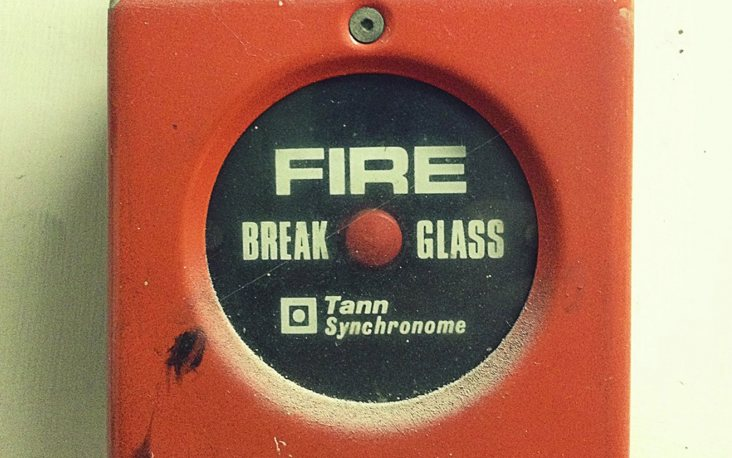
\includegraphics[width=49mm]{level4/challenge11.jpg}
\end{marginfigure}
\subsection{Intro}
In case of fire, break the glass and press the button.

\url{http://46.101.107.117:2204}

Note: The service is restarted every hour at x:00.

\section{Solution}\label{hv22.11solution}

The link takes us to a simple website.  Inspecting the source code leads to a script \verb+script.js+
defining a function \verb+firealert()'+ that writes to the console when the button is pressed.  Look at the console in developer mode and see what is happening:

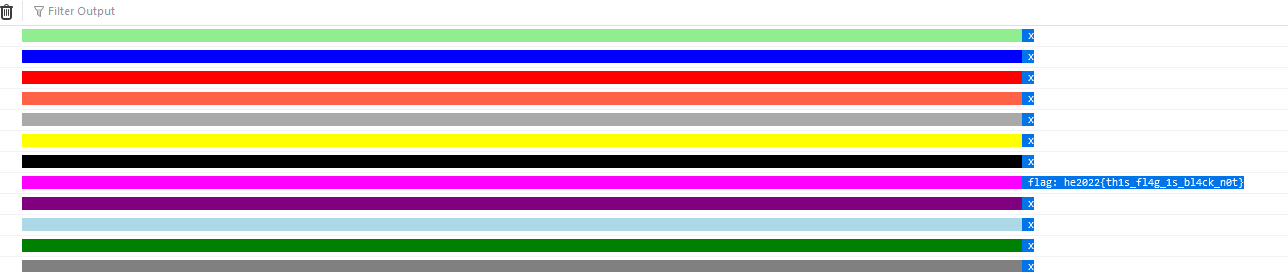
\includegraphics[width=100mm]{level4/solution11.png}

The flag \verb+he2022{th1s_fl4g_1s_bl4ck_n0t}+.




